\documentclass[12pt]{article}
%\usepackage[landscape]{geometry}
\usepackage{hyperref}
\usepackage{graphicx}
\usepackage{subfigure}
\usepackage{amsmath}
\usepackage{amsfonts}
\usepackage{amssymb}
\usepackage{mathrsfs}
\usepackage{bm}
\usepackage{enumitem}
\usepackage{semantic}
\usepackage{empheq}
\usepackage{algorithm}
\usepackage{algpseudocode}
\usepackage{algorithm}

\algnewcommand\algorithmicforeach{\textbf{for each}}
\algdef{S}[FOR]{ForEach}[1]{\algorithmicforeach\ #1\ \algorithmicdo}

\graphicspath{{../}{../results/}{fig/}}
\DeclareGraphicsExtensions{.pdf,.eps,.png,.jpg,.jpeg}

\makeatletter
\newcommand*{\rom}[1]{\expandafter\@slowromancap\romannumeral #1@}
\makeatother

\title{Locality Analysis Against Graph Partitioning}
\date{\today}
\author{CHEN Hongxu\\XU Zhengzi\\NIE Xiao}

\begin{document}
\maketitle
\section{Introduction}

Social media has gained its popularity over the years. According to Pew research center\footnote{\url{http://www.pewinternet.org/data-trend/social-media/social-media-use-all-users}}, $74\%$ of all the Internet users have used the social network sites; and the number keeps increasing. 

Due to the need from the customers, in recent years, many startup companies begin to develop their business in this area. Based on the report of Gust\footnote{\url{https://gust.com/startup-trends}}, a company aims to build the connection between startup and investor, in 2015 second quarter, the number of startups has increased by $20\%$ compared to data at the same time in 2014 and $26\%$ for the first quarter of 2015. Among all the startups, $13\%$ of them mainly focus on providing Internet web services and others, like entertainment applications startups may also include social networking functionalities. 

One of the problems in developing software with social network capability is to divide the user data into groups and store them distributedly. A good way of storing the data will improve the availability by providing replication of the data into different server, and the scalability by maintaining the data locality within the server. Many researchers have developed various complexed partition algorithms to improve the performance of the large networking site. However, few of them have optimised their solution to suit the case where a relatively small network is presented and little resource is available. Therefore, this study is going to evaluate a few well-known partition algorithms' performance for the small startup companies.

\bigskip

The rest of the report is organised in the following way: In section \ref{sec:sec2}, a real world problem is defined with high motivation stated. The next section presents a detailed description of the methodology used in the study. Then the experiment setup and implementation are shown. The results and limitation of the experiment are discussed in section \ref{sec:sec4} and \ref{sec:sec5} respectively. The last section concludes this report by highlight the findings and insights.
\section{Related Work}
\section{Problem Description} \label{sec:sec2}


\subsection{Motivation}

Nowadays, more and more small companies have developed software and mobile applications with networking services. Some of them provide networking function as their main business; while others use it as a method to increase the interaction among their users, and thus attracting more potential users of their products. Those small companies need to store their user profiles into the server. However, many startups may encounter problems where they may be lack of budget to deploy adequate number of servers and other infrastructures. Therefore, they must design their storage algorithm wisely in order to fully utilise their limited resource and achieve a relatively good performance. 

One of the aspects which needs considering is to choose an efficient and effective graph partitioning algorithm to separate the user data and deploy them into different servers. It is important because a good deployment of user data at different server can speed up the query process when user would like to obtain it. Small companies need to provide better user experience in order to survive and thrive. Thus, providing user experience with a fast access rate can help the company to maintain and develop its user base.  

\subsection{Problem Definition}

Our experiment aims to find a suitable graph partition solution for small business which runs networking services. More specifically, we are testing the performance (locality) of different partition algorithms under the same condition, in which we treat any replication of data as overhead. The number of servers is set to a range of small values in order to accord with the real world companies with limited resources. 
\section{Methodology}

\subsection{Algorithms}

In the existing studies of online social networks scalability, we found researchers have developed various partition algorithms to preserve the data locality while reduction the overhead. In this project, we decide to leverage the four graph partition algorithms, namely random partitioning, METIS graph partitioning, community detection algorithm, and SPAR to test the partition performance in the case where different number of server is available.

The social network which need to be partition can be represented by node and edges, where one node specifies one active user in the network, and the edge, which can be directed or indirected, stands for the existence of relationship between the two connected nodes.


\subsubsection{Random Partition}

As the name suggests, random partition algorithm will cluster all the node in a random manner. The possibility for a user node to be stored in a particular server is equal to the possibility for it to be stored in another ones. Since there is no optimization involved in the algorithm, we expected that it will have the highest overhead among all algorithm. Thus, it can server as the baseline for our experiment.  

Another reason for choosing this algorithm is that, since we are focusing on small business with relatively small number of server available, some of the advanced techniques may not function well. Using the random partition algorithm in this situation may reduce the the effort in implementation while achieves similar performance with those advanced algorithm. Even for some large corporation such as facebook, random partition is widely used for simplicity. 

\subsection{Community Detection}

Community detection algorithm bases on the assumption that the input network involves the community structure [1] which can be detected and used as the criteria to perform the partition. The community structure is a network in which nodes can be easily divided into groups/communities in which nodes are densely connected to each other. Whereas the inter-connection between nodes from different group is relatively sparse compared to the intra-connection of nodes within the group.

\begin{figure}[t]
  \centering
  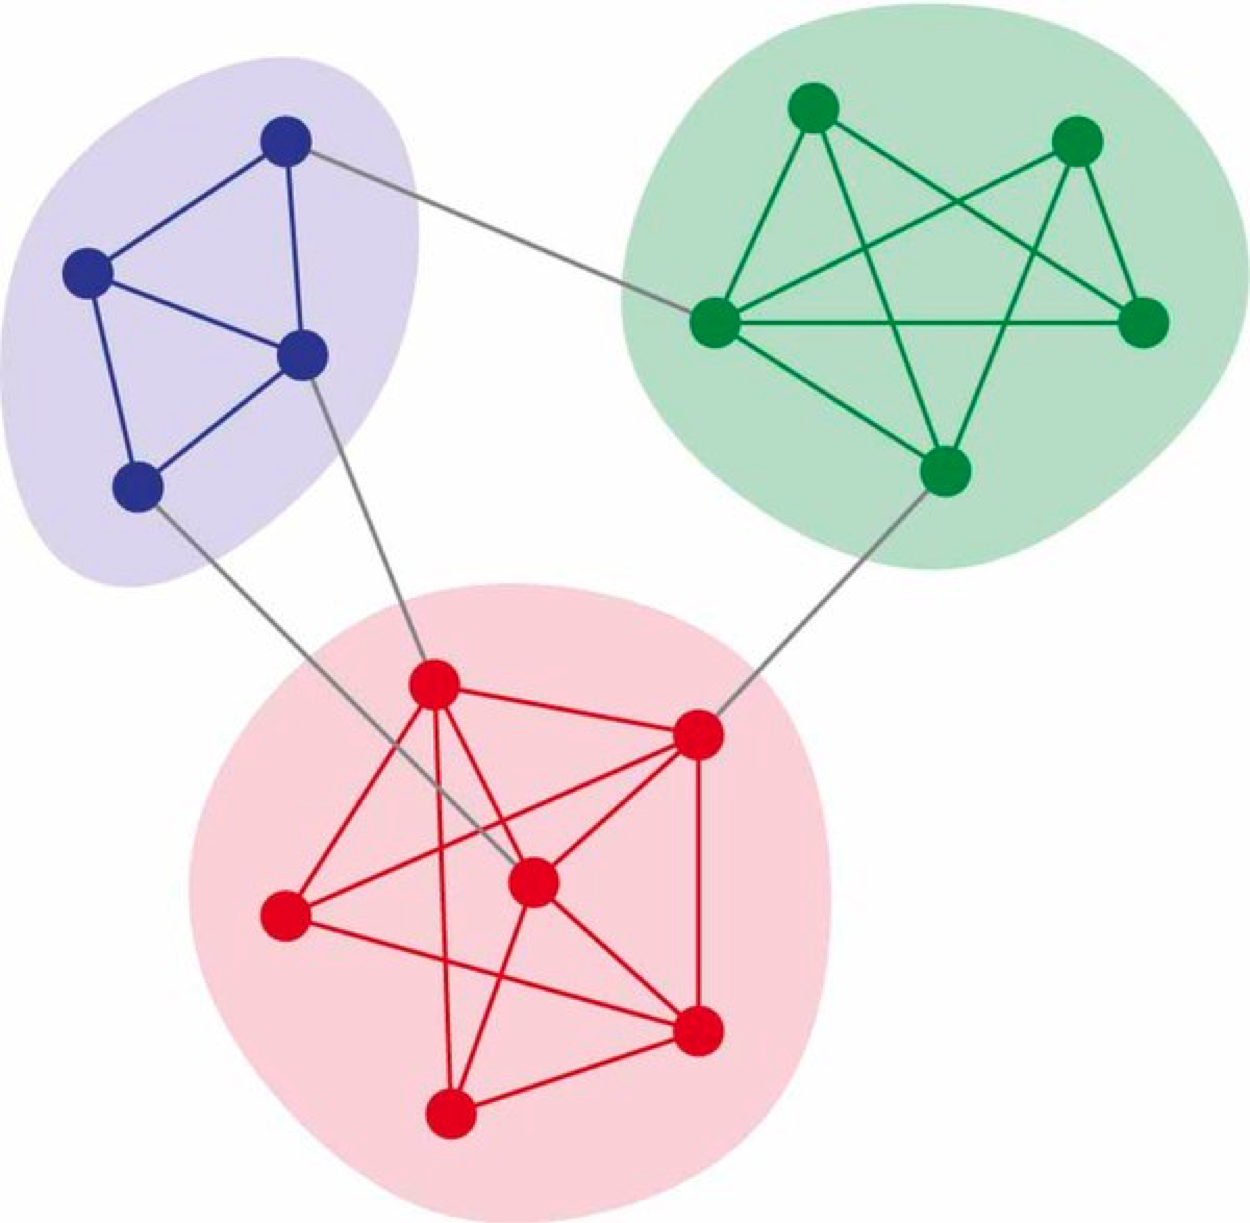
\includegraphics[width=0.6\columnwidth]{cd.png}
  \caption{Community Structure Network}\label{fig:cd}
\end{figure}


Figure 1 has depicted a typical community structure network with three groups. The community detection algorithm tries to identify the structural information in the network and leverage the group information to partition the node. There are various approaches to identify the groups in the network. Each of them has its own advantages in some circumstances. According to Andrea [2], among various community detection algorithm, Infomap [3] has the best performance over the others. In the experiment, we choose the algorithm from xx [4]. Advantages??


\subsection{METIS}

METIS is a multilevel graph partitioning algorithm [1], which consists several stages to partition a large graph. First, it tries to reduce the size of the group by collapsing the nodes and edges. Two similar nodes are grouped together and be represented by a coarser mesh. The coarser mesh then serves as a new large node with weighted edges specify the number of connection between the two meshes. After that, the process is repeated until the graph is small enough for later processing (usually less than $3$k $\sim 5$k nodes). Since the graph is small, METIS then perform a high-cost but high-quality spectral partitioning algorithm on the graph. After the partitioning, a refinement or un-coarsening phase is applied to the graph to retrieve the node back from the mesh recursively. By using the Kernighan-Lin heuristic algorithm [2], METIS can construct back the original graph with an accurate graph partitioning solution.

Figure 2 has given the basic steps of METIS. In the experiment, we used the METIS package from [3]. It is a fast but accurate implementation of METIS which has been used in academic and industrial organizations.

\subsubsection{SPAR}

SPAR is a dynamic graph partitioning algorithm, which guarantees data locality by adding or removing nodes and edges at run time[1]. It makes a balance between the random partition algorithm which costs a lot when it reads the user profile and the full replication algorithm which require more writing operation to the server. SPAR only performs the replication/deletion when a change of the network takes place. In other words, SPAR regards the user's’ action as heuristics to help to build up the node partition layout in the server.

In our experiment, since we use only one replication for every data, whereas SPAR dynamically creates replicas for nodes neighbour in different server, we excluded this method in the experiment. However, the algorithm itself has good performance and may become a choice for the small companies.
\section{Experiment Setup}

\subsection{Data description and Pre-processing}

The whole implementation is available at [6].

\begin{table}[]
\centering
\caption{Basic Graph Information}
\label{my-label}
\begin{tabular}{|c|c|c|c|c|c|}
\hline
\textbf{} & \textbf{\# node} & \textbf{\# edge} & \textbf{clustering} & \textbf{\# triangles} & \textbf{type} \\ \hline
\textbf{Facebook} & 4039 & 88234 & 0.6055 & 1612010 & social \\ \hline
\textbf{DBLP} & 317080 & 1049866 & 0.6324 & 2224385 & \begin{tabular}[c]{@{}c@{}}ground-truth\\ communities\end{tabular} \\ \hline
\textbf{YouTube} & 1134890 & 2987624 & 0.0808 & 3056386 & \begin{tabular}[c]{@{}c@{}}ground-truth\\ communities\end{tabular} \\ \hline
\end{tabular}
\end{table}

\subsection{Comparison of different Partitioning Approaches}

This experiment compares the locality for different partition strategies. Here, we assume that each node in the graph has an equal opportunity to access its neighbors, and additionally each neighbor node is accessed equally. Since we do not apply any replication if the neighbor node is stored remotely, the locality for a single is measured as the ratio of neighbor nodes that are in the same group as the interesting node.
\section{Limitations}

Our partition algorithm performance experiment bears the following limitations.
First, the dataset used in the experiment is retrieved from snap, which provides the so called ego network data. The dataset only represent a small portion of the social network starting from one node and traverse through all of its neighbors. Even the combination of several ego network cannot form a real social network. A real social network map will consist many isolated nodes due to inactive account. By considering the real network layout, in the experiment, will produce more accurate results. 

Second, unlike large social networking site, small companies’ user social network may not exhibit some features such as the community structure among the users. An example is that a mobile online game application company may provide social networking services where the player can make friend in the game. However, the player-to-player interaction is limited to between two players rather than in a group, so that one would like to make friends with someone he does not know and all his friends do not know each other. Therefore, the overall network map will be sparse and even distributed among all the nodes. In this case it is difficult to find a community structure in the networks. In our experiment, the dataset is retrieved from Facebook, DBLP, and YouTube, it may be favorable for some algorithms while make others in disadvantages. In future works, to achieve an unbiased experiment, the user data from small companies needs to be obtained and servers as the input for the testing.

Last, our experiment only considers to store one copy of the user profile into the server.  It is plausible since we are focusing on small business, where the availability of the social networking services may not be a key issue. However, in the real world, some of the companies would like to store the data in several copies. The difference in the number of replication will affect the performance results, for some of the overhead of an algorithm may be considered as a replication stored in a different server. Therefore, the overall overhead decreases when more replication are needed. Future works may take the replication into consideration and get a better performance comparison. 
\section{Conclusion}

In this project, we examined the locality results of a few partitioning algorithms for an existing static network. The experiment has shown that community detection partition achieves the best locality while random partitioning approach has the least computation overhead. If the underlying network is infrequently changed or its size is relatively small, we suggest implementing the METIS algorithm since it leverages the computation and the data locality well. For some companies whose resource is limited, they can opt to choose to combine the random partitioning approach with replication, or some caching mechanisms. Our work also provides a reference for these companies to evaluate the partitioning approaches by themselves.

\bibliographystyle{abbrv}
\bibliography{ref}

\end{document}